\section{Ziel}
\label{sec:Ziel}
In diesem Versuch werden die fundamentalen physikalischen Gesetze der Strahlenoptik untersucht. Dazu werden experimentelle Messwerte mit den theoretisch zu erwartenden
Resultaten vergliechen. Es wird die Beugung, Brechung und Reflexion von monochromatischen Licht betrachtet.
\section{Theorie}
\label{sec:Theorie}
Licht ist eine elektromagnetische Welle. Daher kann Licht in komplexer Weise durch die Maxwell-Gleichungen beschrieben werden. Dies ist für die fundamentalen Gesetze der
Strahlenoptik nicht nötig. Es genügt, Licht auf ein fundamentaleres Verhalten zu vereinfachen. Dazu wird Licht ,aufbauend auf die Überlegungen des niederländischen Physikers 
\textit{Christiaan Huygens}, auf das Ausbreitungsverhalten reduziert. Gemäß des \textit{Huygensschen Prinzips} breitet sich Licht entlang der Wellennormalen aus. Die 
Wellennormale steht immer orthogonal zur \textit{Wellenfront} und ist in \autoref{fig:Huygensbrechung} durch einen roten Pfeil skizziert. Das Huygenssche Prinzip sagt nun aus,
dass sich die Welle ausbreitet, indem an jedem Punkt der Wellenfront eine neue radiale Elementarwelle gleicher Frequenz entsteht. Durch Überlagerung aller dieser Elementarwellen 
ergibt sich eine neue Wellenfront. Dies beschreibt eine gradlinige Propagation einer Lichtwelle ohne Veränderung des Ausbreitungsmediums. Trifft eine Lichtwelle in diesem 
gedanklichen Modell nun auf ein anderes Medium, wird die Welle \textit{gebrochen},\textit{gebeugt} und oder \textit{reflektiert}. Diese Wechselwirkung mit einem
anderen Medium entsteht, da sich Wellen, so auch die Elementarwellen nach Huygens, in unterschiedlichen Medien unterschiedlich schnell ausbreiten. Die drei genannten 
Wechselwirkungen treten dann in Abhänigkeit von den Eigenschaften der Lichtwelle und des Beugungsmaterials auf. 

\begin{figure}
    \centering
    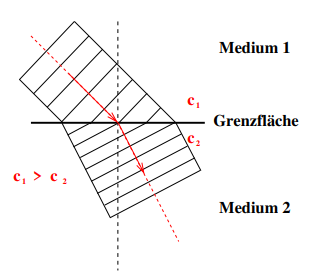
\includegraphics[width=0.5\textwidth]{content/HuygensscheBrechung.png}
    \caption{In dieser Abbildung ist das Huygenssche Prinzip schematisch dargestellt. \cite{v400}.}
    \label{fig:Huygensbrechung}
\end{figure}

\subsection{Reflexion}
\label{subsec:Reflexion}
Nun wird ein Lichtstrahl betrachtet, welcher in einem Winkelintervall von $[\qty{0}{\degree},\qty{90}{\degree}]$ zum Lot auf ein Grenzmedium trifft. Es wird nur der reflektierte Teil
der Lichtwelle betrachtet. Diese Situation ist in \autoref{fig:Reflexion} dargestellt. In dieser Abbildung
beschreibt $\alpha_1$ den Einfallswinkel der Lichtwelle und $\alpha_2$ den \textit{Reflexionswinkel}. Für Reflexion gilt gemäß der Strahlenoptik 
\begin{equation}
  \label{eqn:Reflexionsgesetz}
  \alpha_1 = \alpha_2.
\end{equation}

\begin{figure}
  \centering
  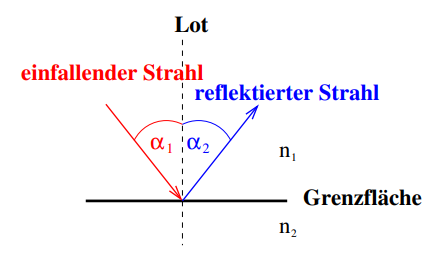
\includegraphics[width=0.5\textwidth]{content/Reflexion.png}
  \caption{In dieser Abbildung wird die Reflexion eines Lichtsstrahles gemäß der Strahlenoptik dargestellt. \cite{v400}.}
  \label{fig:Reflexion}
\end{figure}

\subsection{Brechung}
\label{subsec:Brechung}
Nun wird bei selbiger Ausgangslage der transmitierte Teil des Lichts betrachtet.  
Aufgrund der unterschiedlichen Ausbreitungsgeschwindigkeiten läuft das Licht nun mit einem Brechungswinkel $\beta$ durch das Medium. Diese Situation wird in 
\autoref{fig:Brechung} dargestellt. Dieses Konzept kann ebenfalls aus dem 
Huygenschen Prinzip hergeleitet werden. Nach dem \textit{Snelliusschen Brechungsgesetz} verhalten sich Einfalls- und Brechungswinkel gemäß
\begin{equation}
  \label{eqn:Brechung}
  n_1\sin\alpha = n_2\sin\beta
\end{equation}
zueinander.

\begin{figure}
  \centering
  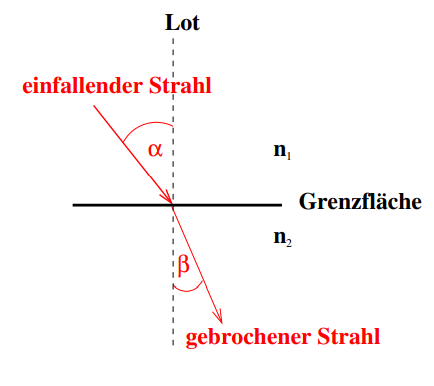
\includegraphics[width=0.5\textwidth]{content/Brechung.png}
  \caption{In dieser Abbildung wird die Brechung eines Lichtsstrahles gemäß der Strahlenoptik dargestellt. \cite{v400}.}
  \label{fig:Brechung}
\end{figure}

Wird nun die Brechung an einem Quader betrachtet fällt auf, dass bei vollständigem Durchlauf eines Lichtstrahls, der austretende Lichtstrahl parallel zum Einfallenden verläuft.
Allerdings erfährt er dabei einen \textit{Strahlenversatz}. Diese Situation kann der \autoref{fig:Strahlenversatz} entnommen werden.
Der Strahlenversatz kann gemäß
\begin{equation}
  \label{eqn:Strahlenversatz}
  s = d\frac{\sin(\alpha - \beta)}{\cos\beta}
\end{equation}
berchnet werden.

\begin{figure}
  \centering
  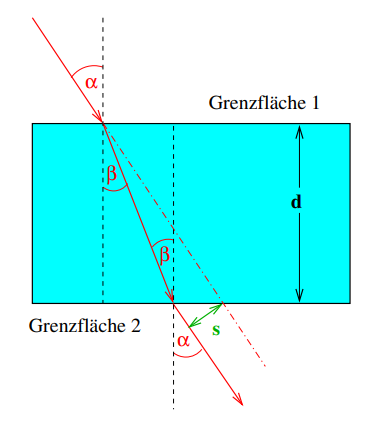
\includegraphics[width=0.5\textwidth]{content/Quader.png}
  \caption{In dieser Abbildung wird der Effekt des Strahlenversatzes dargestellt. \cite{v400}.}
  \label{fig:Strahlenversatz}
\end{figure}

Weiter kann nun auf die Doppelbrechung durch ein Prisma geschlossen werden. Die hierbei entstehende Situation kann \autoref{fig:Prismabrechung} entnommen werden.
Der gesamte Ablenkwinkel $\delta$ kann gemäß 
\begin{equation}
  \label{eqn:delta}
  \delta = (\alpha_1 + \alpha_2) - (\beta_1 + \beta_2)
\end{equation}
berechnet werden.

\begin{figure}
  \centering
  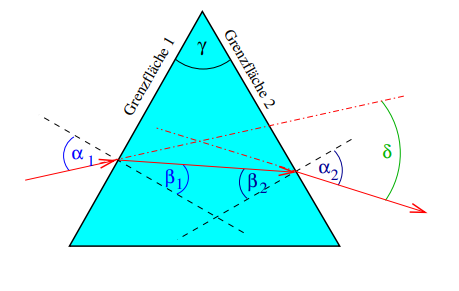
\includegraphics[width=0.5\textwidth]{content/Prismabrechung.png}
  \caption{In dieser Abbildung wird die Doppelbrechung in einem Prisma dargestellt. \cite{v400}.}
  \label{fig:Prismabrechung}
\end{figure}

\subsection{Reflexion und Transmission}
\label{subsec:ReUTra}
In den letzten beiden Abschnitten wurden Transmission und Reflexion voneinander getrennt betrachtet. Allerdings tritt in der Regel meist eine Mischung aus beiden Effekten
auf. Das bedeutet, ein Teil des Strahl wird reflektiert und der andere Teil wird transmitiert und somit gebrochen. Die Gesetze der einzelnen Effekte ändern sich bei Überlagerung
nicht. Allerdings teilt sich die Intensität des einfallenden Strahles in die Intensität des reflektierten- und transmitierten Teils auf. Dabei beschreibt $R$ den Anteil der 
reflektierten Intensität an der einfallenden Intensität und $T$ den Anteil der transmitierten Intensität. Aufgrund der Energieerhaltung muss $R + T = 1$ gelten.

\subsection{Beugung}
\label{subsec:Beugung}
Die Beugung einer Welle kann nicht durch die Strahlenoptik beschrieben werden. Daher wird nun das Phänomen der Beugung durch \textit{Wellenoptik} beschrieben. Licht ist eine
elektromagnetische Welle, weshalb das Superpositionsprinzip gelten muss. Daher können zwei Lichtwellen miteinander interferieren. 
Trifft eine Lichtwelle auf ein Objekt oder einen Spalt, welches oder welcher jeweils klein gegenüber der Wellenlänge ist, tritt
nach der Wechselwirkung ein Interferenzmuster auf einem Schirm auf. Dies bestätigt sich durch einfache Überlegungen gemäß des Huygensschen Gesetzes für eine Welle, welche auf 
einen Spalt trifft. Nun wird nicht nur ein Spalt betrachtet, sondern ein Gitter. Ein Gitter kann vereinfacht als zahlreiche Einzelspalte betrachtet werden. Dabei wird erkannt, 
dass an einem Gitter derselbe Beugungseffekt auftritt. Allerdings treten aufgrund der Anzahl der Einzelspalte nun für jede Wellenlänge Intensitätsmaxima $k$-ter Ordnung auf.
Das Interferenzmuster einer monochromatischen Lichtwelle der Wellenlänge $\lambda$, welche an einem Gitter mit der Gitterkonstante $d$ gebeugt wird, kann in Abhänigkeit vom 
Winkel $\alpha$ durch die Formel
\begin{equation}
  \label{eqn:Beugung}
  d\sin\alpha = k\lambda
\end{equation} 
beschrieben werden.